\documentclass[leqno,aspectratio=169]{beamer}
\usetheme{Madrid}
\usecolortheme{seahorse}

\usepackage[linesnumbered,algoruled,boxed,lined]{algorithm2e}
\usepackage{amsfonts,amsmath,amsthm}
\usepackage{bm}
\usepackage{booktabs}
\usepackage{caption}
\usepackage{color}
\usepackage{graphicx}
\graphicspath{{./}{../image/}} % graphic path
\usepackage{hyperref}
\hypersetup{colorlinks,citecolor=blue,linkcolor=[RGB]{50,50,172}}
\usepackage{multicol}
\usepackage{multirow}
\usepackage[authoryear]{natbib}
\usepackage{setspace}
\usepackage{soul}
\usepackage{textpos}
\usepackage{tikz}

%% notations
\newcommand{\blue}[1]{\textcolor{blue}{#1}}
\newcommand{\red}[1]{\textcolor{red}{#1}}
\newcommand{\bmI}{\bm{I}}
\newcommand{\bmOmega}{\bm{\Omega}}
\newcommand{\bmSigma}{\bm{\Sigma}}
\newcommand{\bmS}{\bm{S}}
\newcommand{\bmW}{\bm{W}}
\newcommand{\bmX}{\bm{X}}
\newcommand{\bmY}{\bm{Y}}
\newcommand{\bmZ}{\bm{Z}}
\newcommand{\bmbeta}{\bm{\beta}}
\newcommand{\hatbmOmega}{\hat{\bm{\Omega}}}
\newcommand{\tr}{\text{tr}}
\DeclareMathOperator*{\argmin}{arg \, min}

% consistent with R manual
\newcommand\pkg[1]{\texttt{#1}}
\let\proglang=\textsf \let\code=\texttt

\setbeamercovered{transparent}
\setbeamertemplate{caption}[numbered]
\setbeamertemplate{enumerate item}[default]
\setbeamertemplate{itemize item}[circle]
\setbeamertemplate{section in toc}[default]
\setbeamertemplate{subsection in toc}[default]

\AtBeginSection[]{
\begin{frame}<beamer>{Overview}
\tableofcontents[currentsection]
\end{frame}}


\title[\textcolor{black}{FCABN}]{
{\bf \normalsize Title}}
%\subtitle[]{}
\author[Xiaohang Ma, Shiying Xiao, Xiaohui Yin]{\bf
	Xiaohang Ma\textsuperscript{1},
	Shiying Xiao\textsuperscript{2},
	Xiaohui Yin\textsuperscript{2}}
\institute[UConn]{
\textsuperscript{1}{\small Department of Mathematics, University of Connecticut}
\\
\textsuperscript{2}{\small Department of Statistics, University of Connecticut}
}
\date[October 7, 2024]{
{\small Storrs, CT} \\
{\small October 7, 2024}}

\begin{document}

\begin{frame}[plain]
\titlepage
\end{frame}

\addtobeamertemplate{frametitle}{}{
\begin{textblock*}{70mm}(.9\textwidth,-0.65cm)

\includegraphics[width=.2\textwidth]{uconn-wordmark-single-blue.png}
\end{textblock*}}


\begin{frame}
\frametitle{Overview}
\tableofcontents
\end{frame}


\section[Introduction]{Introduction}

\begin{frame}
\frametitle{Motivations}
\begin{itemize}
\item Functional magnetic resonance imaging (fMRI), especially resting-state 
fMRI, is crucial for understanding brain interactions and neurological diseases 
like Alzheimer's disease (AD).
\bigskip
\item Recent studies combine fMRI and tau-PET imaging to link brain 
architecture with tau protein accumulation, a key feature of AD.
\bigskip
\item Network-based functional connectivity analysis methods have emerged as a 
powerful tool for exploring interactions among brain regions.
\bigskip
\item A comprehensive examination of the methods has been lacking.
\end{itemize}
\end{frame}

%\section{Literature Review}
\subsection{Environment Invariant Linear Least Squares, \cite{fan2023environmentinvariantlinearsquares}}
\section{Introduction}
\begin{frame}
  \frametitle{Motivating Example: Risks of Using Spurious Variables}
   A task to classify cows and camels based on extracted hierarchical features: 
  \begin{itemize}
  \item There is a dataset $\mathcal D$ containing 10k images of cows and camels from the Internet. When Using 70\% to train the classifier, top two features are the back shape $x_1$, and the background color $x_2$, and it performs well on the remaining 30\% testing set. It is contemplated that cows often appear on the grass while most camels appear on the sand from this dataset.
  \end{itemize}
  \vspace{6pt}
  \centering
  \begin{minipage}{.3\textwidth}
    \begin{figure}[H]
      \centering 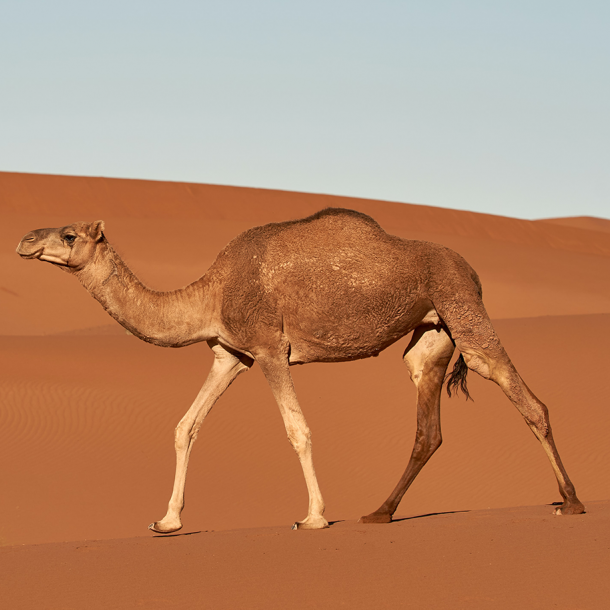
\includegraphics[width=0.8\textwidth]{figs/camel_sand.png}
      \caption{Camel in brown}
    \end{figure}
  \end{minipage}% This must go next to `\end{minipage}`
  \begin{minipage}{.3\textwidth}
    \begin{figure}[H]
      \centering 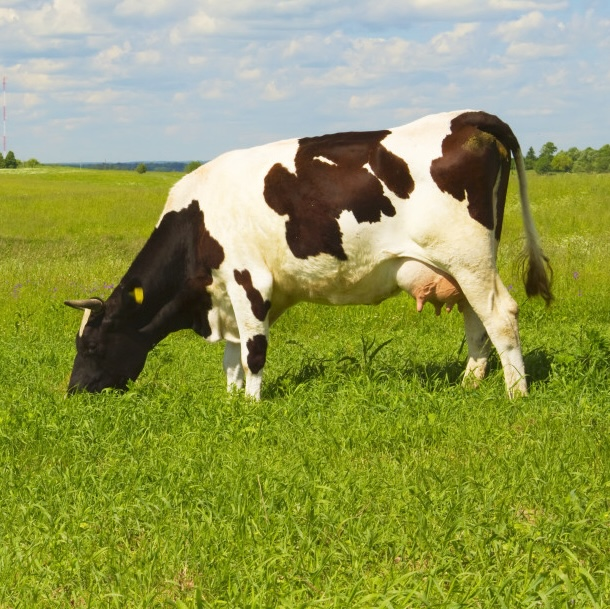
\includegraphics[width=0.8\textwidth]{figs/cow_grass.jpg}
      \caption{Cow in green}
    \end{figure}
  \end{minipage}
\end{frame}

\begin{frame}
  \frametitle{Motivating Example (Cond)}
  \begin{itemize}
  \item However, introducing $x_2$ is not what we expected: the classifier can not work well in a place farming camels and cows, in which the background color is fixed.
  \item If we have another dataset $\widetilde {\mathcal D}$, in which the association between the background color and object label still exists yet slightly perturbs. Intuitively, we may infer that $x_2$ may be a ``spurious'' variable for prediction or causation.
  \end{itemize}
  \vspace{6pt}
  \centering
  \begin{minipage}{.3\textwidth}
    \begin{figure}[H]
      \centering 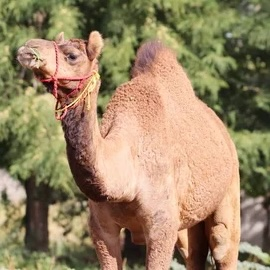
\includegraphics[width=0.8\textwidth]{figs/camel_grass}
      \caption{Camel in green}
    \end{figure}
  \end{minipage}% This must go next to `\end{minipage}`
  \begin{minipage}{.3\textwidth}
    \begin{figure}[H]
      \centering 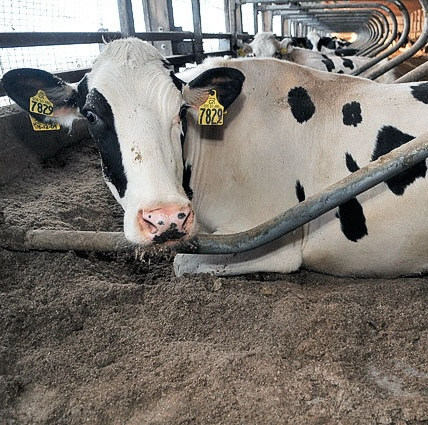
\includegraphics[width=0.8\textwidth]{figs/cow_sand.jpeg}
      \caption{Cow in brown}
    \end{figure}
  \end{minipage}
\end{frame}


\begin{frame}
  \frametitle{Some Definition}
  This paper propose the multiple-environment version of linear least squares. It utilizes the heterogeneity across datasets.
  It combines the linear least squares solutions across different datasets and uses their differences to determine the true parameter and important variables in a completely data-driven manner.
  
  \vspace{8pt}
  
  Here are some definitions needed: 
    \begin{itemize}
    \item response variable $y \in \mathbb R$
    \item explanatory variable $\bm x \in \mathbb R^p$
    \item set of environments $\mathcal E$
    \item observations from environment $e\in \mathcal E$:
      $(\bm x_1^{(e)}, y_1^{(e)}), \dots,  (\bm x_n^{(e)}, y_n^{(e)}) \sim \mu^{(e)}$
    \end{itemize}
    
\end{frame}

\begin{frame}
  \frametitle{Model Formulation}
  The true linear model is assumed as
  \begin{align}
    \label{main_eq}
    y^{(e)} = (\bm\beta^*_{S^*})^\top \bm x_{S^*}^{(e)} + \varepsilon^{(e)} ~~~~~ \text{with} ~~~~ \mathbb{E}[\varepsilon^{(e)}|\bm x_{S^*}^{(e)}] \equiv 0,
  \end{align} where the unknown set of important variables $S^* = \{j: \beta_j^* \neq 0\}$ and the model parameters $\bm \beta^*$ are the same across different environments, while $\mu^{(e)}$, the distribution of $(\bm x^{(e)},y^{(e)})$, may vary.
  
  \vspace{8pt}

  The aim is to estimate $\bm\beta^*$ and $S^*$ using the $n\cdot |\mathcal{E}|$ data $\{(\bm x_i^{(e)}, y_i^{(e)})\}_{e\in \mathcal{E}, i\in \{1,\ldots, n\}}$.
\end{frame}

\begin{frame}
  \frametitle{Challenges}
  \begin{itemize}
  \item $\bm \beta^*$ is mot the best linear predictor for each single environment.
  \item A smaller mean squared error by incorporating the linear spurious variables $\bm x_{S^{*\perp}}$ defined outside the set of important variables for all environments.
    $\bm x_{S^{*\perp}}^{(e)}$ can capture information in $\varepsilon^{(e)}$.
  \item Such spurious variables are not stable when generalized to other environments, because the association between these variables and $y$ are not stable. (background color in the motivating example)
  \end{itemize}
\end{frame}

\begin{frame}
  \frametitle{Loss Function}
  The population-level EILLS objective is 
  \begin{scriptsize}
  \begin{align*}
    \mathsf{Q}_\gamma(\bm\beta) &= \underbrace{\sum_{e\in \mathcal{E}} \mathbb{E} \left[|y^{(e)} - \bm\beta^\top \bm x^{(e)}|^2\right]}_{\mathsf{R}(\bm\beta)} \nonumber\\
                                &\qquad + \gamma \underbrace{\sum_{j=1}^p \mathbf{1}\{\beta_j\neq 0\} \times  \sum_{e\in \mathcal{E}}  \left|\mathbb{E} [(y^{(e)} - \bm\beta^\top \bm x^{(e)}) x_j^{(e)}]\right|^2}_{\mathsf{J}(\bm\beta)},
  \end{align*}
  \end{scriptsize}
  where $\gamma$ is a tuning parameter.
  \begin{itemize}
  \item $\mathsf R(\bm\beta)$ requires a good overall solution in each single environment.
  \item $\mathsf J(\bm\beta)$ discourages selecting variables that have strong correlation with the fitted residuals in some environments.
  \item From computational perspective, we have
    \begin{align*}
    \mathsf{J}(\bm \beta) &= \sum_{j=1}^p \mathbf{1}\{\beta_j \neq 0\} \sum_{e\in \mathcal{E}} \frac{1}{4} |\nabla_j \mathsf{R}^{(e)}(\bm\beta)|^2,
  \end{align*}
  \end{itemize}
\end{frame}

\begin{frame}
  \frametitle{Empirical Loss Function}
  \begin{align*}
    \hat{\mathsf{J}}(\bm\beta) &= \sum_{j=1}^p \mathbf{1}\{\beta_j \neq 0\} \sum_{e\in \mathcal{E}}  \left| \hat{\mathbb{E}}[x_j^{(e)} (y^{(e)} - \bm\beta^\top \bm x^{(e)})]\right|^2\\
    \hat{\mathsf{R}}(\bm\beta)& = \sum_{e\in \mathcal{E}}  \frac{1}{n^{(e)}} \sum_{i=1}^{n^{(e)}} \{ y^{(e)}_i - \bm\beta^\top \bm x^{(e)}_i \}^2\\
    \hat{\mathsf{Q}}(\bm\beta,\gamma) &= \hat{\mathsf{R}}(\bm\beta) + \lambda \hat{\mathsf{J}}(\bm\beta)
  \end{align*}
  Some linear exogenous variables which do not contribute to explaining $y$ can
  be eliminated further by introducing an $l_0$ penalty as
    \begin{align*}
   \hat{\mathsf{L}}(\bm\beta,\gamma,\lambda) =  \hat{\mathsf{R}}(\bm\beta) + \lambda \hat{\mathsf{J}}(\bm\beta) + \lambda \|\bm\beta\|_0.
  \end{align*}
\end{frame}

\begin{frame}
  \frametitle{An Illustration}
  \begin{figure}[H]
      \centering 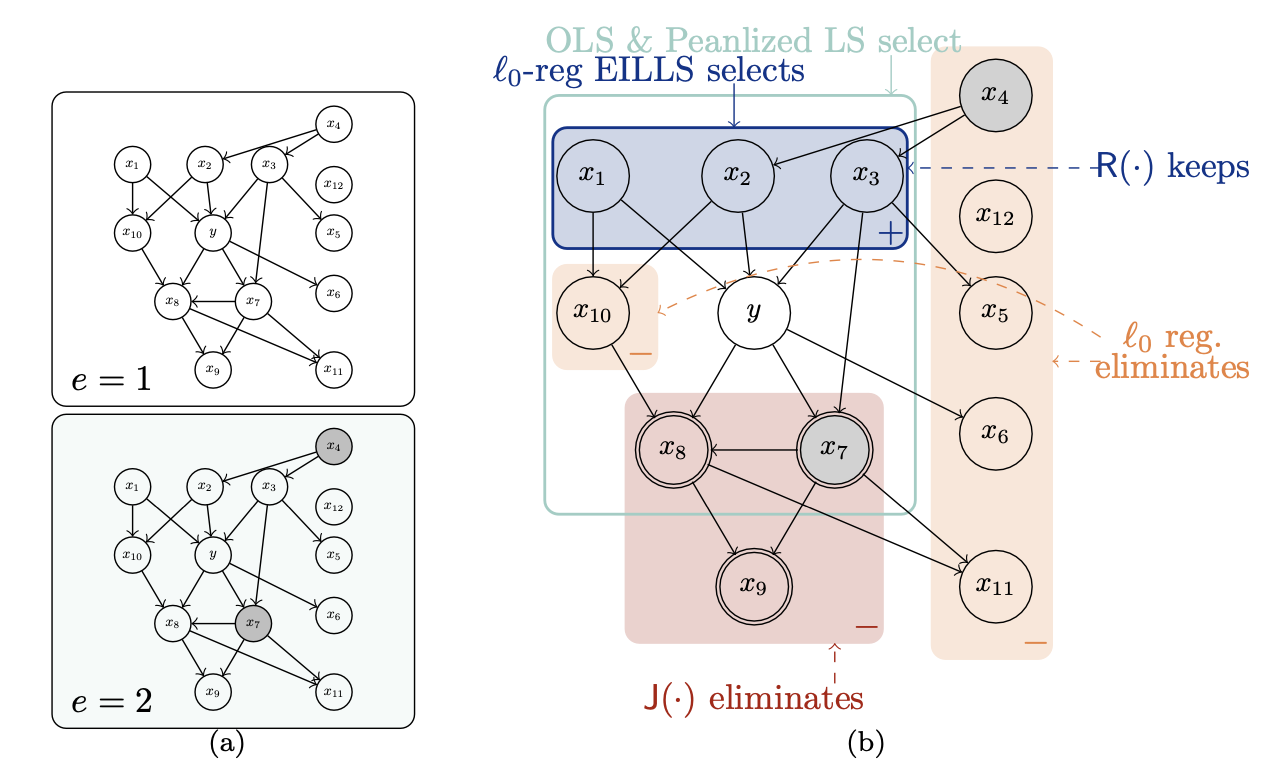
\includegraphics[width=0.8\textwidth]{figs/example}
      \caption{An Example for Illustration, figure from \cite{fan2023environmentinvariantlinearsquares}}
    \end{figure}
\end{frame}
%%% Local Variables:
%%% mode: latex
%%% TeX-master: "proposal"
%%% End:


\begin{frame}[allowframebreaks]
\frametitle{References}
\bibliographystyle{plain}
\bibliography{bib}
\end{frame}

\end{document}
%%% Local Variables:
%%% mode: latex
%%% TeX-master: t
%%% End:
